\section{Unifikace}\label{section:unification}

Místo substitucí \alert{všech} základních termů a práce s touto novou, obrovskou a typicky nekonečnou množinou klauzulí, je lepší najít v konkrétním rezolučním kroku `vhodnou' substituci a pracovat jen s ní. V této sekci vysvětlíme, co znamená `vhodná' (tzv. \alert{unifikace}) a jak ji lze hledat (pomocí \alert{unifikačního 
algoritmu}).

\subsection{Substituce}
%\todo change terms of sigma to s and tau to t?

Nejprve uveďme několik příkladů `vhodných' substitucí:

\begin{example}\label{example:substitutions}
\begin{itemize}
    \item Z klauzulí $\{P(x),Q(x,a)\}$ a $\{\neg P(y),\neg Q(b,y)\}$ získáme pomocí substituce $\{x/b,y/a\}$ klauzule $\{P(b),Q(b,a)\}$ a $\{\neg P(a),\neg Q(b,a)\}$, a z nich potom rezolucí klauzuli $\{P(b),\neg P(a)\}$. Mohli bychom také použít substituci $\{x/y\}$ a rezolucí přes $P(y)$ získat rezolventu $\{Q(y,a),\neg Q(b,y)\}$.
    \item Máme-li klauzule $\{P(x),Q(x,a),Q(b,y)\}$ a $\{\neg P(v),\neg Q(u,v)\}$, vhodnou substitucí je $\{x/b,y/a,u/b,v/a\}$; dostáváme $\{P(b),Q(b,a)\}$ a $\{\neg P(a),\neg Q(b,a)\}$, jejichž rezolventou je $\{P(b),\neg P(a)\}$.
    \item Podívejme se ještě na klauzule $\{P(x),Q(x,z)\}$ a $\{\neg P(y),\neg Q(f(y),y)\}$. Mohli bychom použít substituci $\{x/f(a),y/a,z/a\}$ a získat tak dvojici klauzulí $\{P(f(a)),Q(f(a),a)\}$ a $\{\neg P(a),\neg Q(f(a),a)\}$, rezolucí potom $\{P(f(a)),\neg P(a)\}$.
    
    Lepší ale bude využít substituce $\{x/f(z),y/z\}$, po které máme $\{P(f(z)),Q(f(z),z)\}$ a $\{\neg P(z),\neg Q(f(z),z)\}$, a rezolventu $\{P(f(z)),\neg P(z)\}$. Tato substituce je \alert{obecnější}, a výsledná rezolventa `říká více' než $\{P(f(a)),\neg P(a)\}$ (ta je jejím důsledkem, ale naopak to neplatí).
\end{itemize}
\end{example}

Nyní zavedeme potřebnou terminologii týkající se substitucí. Substituce budeme aplikovat na termy nebo na literály (atomické formule nebo jejich negace), označme tyto dohromady jako \alert{výrazy}. 

\begin{definition}[Substituce]
    \alert{Substituce} je konečná množina $\sigma=\{x_1/t_1,\dots,x_n/t_n\}$, kde $x_i$ jsou navzájem různé proměnné a $t_i$ jsou termy, přičemž vyžadujeme, aby term $t_i$ nebyl roven proměnné $x_i$. Substituce $\sigma$ je 
    \begin{itemize}
        \item \alert{základní}, jsou-li všechny termy $t_i$ konstantní,
        \item \alert{přejmenování proměnných}, jsou-li všechny termy $t_i$ navzájem různé proměnné.
    \end{itemize}
    \alert{Instance} výrazu (termu nebo literálu) $E$ \alert{při substituci $\sigma=\{x_1/t_1,\dots,x_n/t_n\}$} je výraz vzniklý z $E$ simultánním nahrazením všech výskytů proměnných $x_i$ termy $t_i$, označme jej $E\sigma$. Je-li $S$ množina výrazů, potom značíme $S\sigma=\{E\sigma\mid E\in S\}$.
\end{definition}

Protože proměnné nahrazujeme \alert{simultánně} pro všechny proměnné zároveň, případný výskyt proměnné $x_i$ v termu $t_j$ nepovede ke zřetězení substitucí.

\begin{example}
Například pro $S=\{P(x),R(y,z)\}$ a substituci $\sigma=\{x/f(y,z),y/x,z/c\}$ máme:
$$
S\sigma=\{P(f(y,z)),R(x,c)\}
$$
\end{example}

Substituce můžeme přirozeně \alert{skládat}. Složení substitucí $\sigma$ a $\tau$, kde nejprve aplikujeme $\sigma$ a potom~$\tau$, budeme zapisovat jako $\sigma\tau$. Bude tedy platit $E(\sigma\tau)=(E\sigma)\tau$, pro libovolný výraz~$E$.

\begin{example}\label{example:compose-substitutions}
    Začněme opět příkladem. Máme-li výraz $E=P(x,w,u)$, a substituce \begin{align*}
        \sigma&=\{x/f(y),w/v\}\\
        \tau&=\{x/a,y/g(x),v/w,u/c\}
    \end{align*}
    potom je $E\sigma=P(f(y),v,u)$ a $(E\sigma)\tau=P(f(g(x)),w,c)$.
    Musí tedy platit: 
    $$
    \sigma\tau=\{x/f(g(x)),y/g(x),v/w,u/c\}
    $$
\end{example}

Nyní formální definice:

\begin{definition}[Skládání substitucí]
Mějme substituce $\sigma=\{x_1/t_1,\dots,x_n/t_n\}$ a $\tau=\{y_1/s_1,\dots,y_m/s_m\}$. \alert{Složení substitucí $\sigma$ a $\tau$} je substituce
$$
\sigma\tau=\{x_i/t_i\tau\mid x_i\in X,x_i\neq t_i\tau\}\cup\{y_j/s_j\mid y_j\in Y\setminus X\}
$$
kde $X=\{x_1,\dots,x_n\}$ a $Y=\{y_1,\dots,y_m\}$.
\end{definition}

Všimněte si, že skládání substitucí není komutativní, $\sigma\tau$ je typicky zcela jiná substituce než $\tau\sigma$.

\begin{example}
    Jsou-li $\sigma$ a $\tau$ jako v Příkladu \ref{example:compose-substitutions}, potom: 
    $$
    \tau\sigma=\{x/a,y/g(f(y)),u/c,w/v\}\neq \sigma\tau
    $$
\end{example}

Nyní ukážeme, že takto definované skládání substitucí splňuje požadovanou vlastnosti, a také že je \alert{asociativní}. Z asociativity plyne, že nemusíme (a také nebudeme) psát závorky ve složení $\sigma\tau\varrho$, $\sigma_1\sigma_2\cdots\sigma_n$ apod.

\begin{proposition}
Mějme substituce $\sigma$, $\tau$, $\varrho$, a libovolný výraz $E$. Potom platí:
\begin{enumerate}[(i)]
    \item $(E\sigma)\tau=E(\sigma\tau)$
    \item $(\sigma\tau)\varrho=\sigma(\tau\varrho)$
\end{enumerate}
\end{proposition}

\begin{proof}
Nechť $\sigma=\{x_1/t_1,\dots,x_n/t_n\}$ a $\tau=\{y_1/s_1,\dots,y_m/s_m\}$. Stačí dokázat v případě, kdy výraz $E$ je jediná proměnná, zbytek snadno plyne indukcí. (Substituce nijak nemění ostatní symboly.) Rozdělíme na tři případy:
\begin{itemize}
    \item Je-li $E=x_i$ pro nějaké $i$, potom $E\sigma=t_i$ a $(E\sigma)\tau=t_i\tau=E(\sigma\tau)$, kde druhá rovnost je z definice $\sigma\tau$.
    \item Je-li $E=y_j$ pro nějaké $j$, potom $E\sigma=E$ a $(E\sigma)\tau=E\tau=s_j=E(\sigma\tau)$ opět z definice $\sigma\tau$.
    \item Je-li $E$ jiná proměnná, potom $(E\sigma)\tau=E=E(\sigma\tau)$.
\end{itemize}
Tím jsme dokázali (i). Asociativitu (ii) snadno dokážeme opakovaným užitím (i). Následující platí pro každý výraz $E$, tedy i pro každou proměnnou:
$$
E((\sigma\tau)\varrho)=(E(\sigma\tau))\varrho=((E\sigma)\tau)\varrho=(E\sigma)(\tau\varrho)=E(\sigma(\tau\varrho)).
$$
Z toho plyne, že $(\sigma\tau)\varrho$ a $\sigma(\tau\varrho)$ jsou touž substitucí.\footnote{Podrobněji: používáme zřejmou vlastnost, že pro substituci $\pi$ platí $\pi=\{z_1/v_1,\dots,z_k/v_k\}$, právě když $E\pi=v_i$ pro $E=z_i$  a $E\pi=E$ je-li $E$ proměnná různá od všech $z_i$.}
\end{proof}    

\subsection{Unifikační algoritmus}

Které substituce jsou tedy `vhodné'? Takové, po jejichž provedení se dané výrazy `stanou stejnými', tj. \alert{unifikovanými} (viz Příklad \ref{example:substitutions}).

\begin{definition}[Unifikace]
    Mějme konečnou množinu výrazů $S=\{E_1,\dots,E_n\}$. Substituce $\sigma$ je \alert{unifikace pro $S$}, pokud $E_1\sigma=E_2\sigma=\cdots =E_n\sigma$, neboli $S\sigma$ obsahuje jediný výraz. Pokud existuje, potom říkáme také, že $S$ je \alert{unifikovatelná}. 
    
    Unifikace pro $S$ je \alert{nejobecnější}, pokud pro každou unifikaci $\tau$ pro $S$ existuje substituce $\lambda$ taková, že $\tau=\sigma\lambda$. Všimněte si, že nejobecnějších unifikací pro $S$ může být více, ale liší se jen přejmenováním proměnných.
\end{definition}

\begin{example}
   Uvažme množinu výrazů $S=\{P(f(x),y),P(f(a),w)\}$. Nejobecnější unifikací pro $S$ je $\sigma=\{x/a,y/w\}$. Jinou unifikací je např. $\tau=\{x/a,y/b,w/b\}$, není ale nejobecnější, nelze z ní získat např. unifikaci $\varrho=\{x/a, y/c, w/c\}$. Unifikaci $\tau$ naopak lze získat z nejobecnější unifikace $\sigma$, a to pomocí substituce $\lambda=\{w/b\}$: $\tau=\sigma\lambda$
\end{example}

Nyní představíme \alert{unifikační algoritmus}. Jeho vstupem je neprázdná, konečná množina výrazů $S$, a výstupem je buď nejobecnější unifikace pro $S$, nebo informace, že $S$ není unifikovatelná. Algoritmus postupuje od začátku výrazů a postupně aplikuje substituce tak, aby se výrazy stávaly více podobnými. Potřebujeme následující definici:

Nechť $p$ je první (nejlevější) pozice, na které se nějaké dva výrazy z $S$ liší. Potom \alert{neshoda v $S$}, označme $D(S)$, je množina všech podvýrazů začínajících na pozici $p$ výrazů z $S$.

\begin{example}
Pro $S=\{P(x,y),P(f(x),z),P(z,f(x))\}$ je $p=3$ a $D(S)=\{x,f(x),z\}$.  
\end{example}

\begin{algorithm}[Unifikační algoritmus]{\,}
\begin{itemize}
    \item \textbf{vstup}: konečná množina výrazů $S\neq\emptyset$,
    \item \textbf{výstup:} nejobecnější unifikace $\sigma$ pro $S$ nebo informace, že $S$ není unifikovatelná
\end{itemize}
\begin{enumerate}[(1)]\setcounter{enumi}{-1}
    \item nastav $S_0:=S$, $\sigma_0:=\emptyset$, $k:=0$
    \item pokud $|S_k|=1$, vrať $\sigma=\sigma_0\sigma_1\cdots \sigma_k$
    \item zjisti, zda v $D(S_k)$ existuje proměnná $x$ a term $t$ \alert{neobsahující} $x$
    \item pokud ano, nastav $\sigma_{k+1}:=\{x/t\}$, $S_{k+1}:=S_k\sigma_{k+1}$, $k:=k+1$, a jdi na (1)
    \item pokud ne, odpověz, že $S$ není unifikovatelná
\end{enumerate}
\end{algorithm}

\begin{remark}
    Hledání proměnné $x$ a termu $t$ v kroku (2) může být relativně výpočetně náročné.
\end{remark}

Než se pustíme do důkazu korektnosti, ukážeme si běh algoritmu na příkladě

\begin{example}
Aplikujme unifikační algoritmus na následující množinu: 
$$
S=\{P(f(y,g(z)),h(b)),\ P(f(h(w),g(a)),t),\ P(f(h(b),g(z)),y)\}
$$
\begin{itemize}
    \item[($k=0$)] Množina $S_0=S$ není jednoprvková, $D(S_0)=\{y,h(w),h(b)\}$ obsahuje term $h(w)$ a proměnnou $y$ nevyskytující se v $h(w)$. Nastavíme $\sigma_1=\{y/h(w)\}$ a $S_1=S_0\sigma_1$, tj. máme:
    
    $$S_1=\{P(f(h(w),g(z)),h(b)),\ P(f(h(w),g(a)),t),\ P(f(h(b),g(z)),h(w))\}$$

    \item[($k=1$)] $D(S_1)=\{w,b\}$, $\sigma_2=\{w/b\}$, $S_2=S_1\sigma_2$, tj.
    
    $$S_2=\{P(f(h(b),g(z)),h(b)),\ P(f(h(b),g(a)),t)\}$$
        
    \item[($k=2$)] $D(S_2)=\{z,a\}$, $\sigma_3=\{z/a\}$, $S_3=S_2\sigma_3$, tj.
    
    $$S_3=\{P(f(h(b),g(a)),h(b)),\ P(f(h(b),g(a)),t)\}$$

    \item[($k=3$)] $D(S_3)=\{h(b),t\}$, $\sigma_4=\{t/h(b)\}$, $S_4=S_3\sigma_4$, tj.
    
    $$S_4=\{P(f(h(b),g(a)),h(b))\}$$

    \item[($k=4$)] $S_4$ je jednoprvková, nejobecnější unifikace pro $S$ je následující:
    
    $$
    \sigma=\sigma_1\sigma_2\sigma_3\sigma_4=\{y/h(w)\}\{w/b\}\{z/a\}\{t/h(b)\}=\{y/h(b),w/b,z/a,t/h(b)\}
    $$
\end{itemize}     
\end{example}

\begin{proposition}\label{proposition:unification-algorithm}
Unifikační algoritmus je korektní. Pro každý vstup $S$ skončí v konečně mnoha krocích, a je-li $S$ unifikovatelná, odpoví nejobecnější unifikaci $\sigma$, jinak odpoví, že $S$ není unifikovatelná.

Je-li $S$ unifikovatelná, potom pro sestrojenou nejobecnější unifikaci $\sigma$ navíc platí, že je-li $\tau$ libovolná unifikace, potom $\tau=\sigma\tau$.
\end{proposition}
\begin{proof}
V každém kroku $k$ eliminujeme nějakou proměnnou, algoritmus tedy musí skončit. Pokud algoritmus skončí neúspěchem v kroku $k$, potom nelze unifikovat množinu $S_k$. Lze snadno nahlédnout, že v tom případě nelze unifikovat ani $S$.

Pokud algoritmus odpoví $\sigma=\sigma_0\sigma_1\cdots\sigma_k$, zjevně jde o unifikaci. Zbývá dokázat, že je nejobecnější, k tomu stačí dokázat silnější vlastnost (`navíc') popsanou v tvrzení.

Mějme libovolnou unifikaci $\tau$ pro $S$. Ukážeme indukcí, že pro každé $0\leq i\leq k$ platí:
$$
\tau=\sigma_0\sigma_1\cdots\sigma_i\tau
$$
Pro $i=0$ je $\sigma_0=\emptyset$ a $\tau=\sigma_0\tau$ tedy platí triviálně. Předpokládejme, že to platí pro nějaké $i$, a dokažme pro $i+1$. Nechť $\sigma_{i+1}=\{x/t\}$. Stačí dokázat, že pro libovolnou proměnnou $u$ platí: 
$$
u\sigma_{i+1}\tau=u\tau
$$
Z toho už okamžitě plyne i $\tau=\sigma_0\sigma_1\cdots\sigma_i\sigma_{i+1}\tau$.

Je-li $u\neq x$, potom $u\sigma_{i+1}=u$, tedy i $u\sigma_{i+1}\tau=u\tau$. V případě $u=x$ máme $u\sigma_{i+1}=x\sigma_{i+1}=t$. Protože $\tau$ unifikuje množinu $S_i=S\sigma_0\sigma_1\cdots\sigma_i$, a proměnná $x$ i term $t$ jsou v neshodě $D(S_i)$, musí $\tau$ unifikovat $x$ a $t$. Jinými slovy, $t\tau=x\tau$, neboli $u\sigma_{i+1}\tau=u\tau$, což jsme chtěli dokázat.
\end{proof}


\section{Rezoluční metoda}\label{section:predicate-resolution-method}

Chceme-li dokázat, že $T\models\varphi$, umíme díky Skolemizaci najít CNF formuli $S$, která je nesplnitelná, právě když je nesplnitelná teorie $T\cup\{\neg\varphi\}$, neboli právě když $T\models\varphi$. Stačí tedy najít rezoluční zamítnutí $S$.

V této sekci popíšeme vlastní rezoluční metodu. Většina pojmů i tvrzení bude velmi podobná výrokové logice. Jediným podstatným rozdílem bude \alert{rezoluční pravidlo}.


\subsection{Rezoluční pravidlo}

Rezolventou dvojice klauzulí bude klauzule, kterou z nich lze odvodit aplikací \alert{(nejobecnější) unifikace}. Nejprve příklad:

\begin{example}
Mějme klauzule $C_1=\{P(x),Q(x,y),Q(x,f(z))\}$ a $C_2=\{\neg P(u),\neg Q(f(u),u)\}$. Vyberme z první \alert{oba} pozitivní literály začínající $Q$ a ze druhé negativní literál začínající $\neg Q$. Množinu výrazů $S=\{Q(x,y),Q(x,f(z)),Q(f(u),u)\}$ lze unifikovat pomocí nejobecnější unifikace $\sigma=\{x/f(f(v)),y/f(v),z/v,u/f(v)\}$. Po aplikaci této unifikace získáme klauzule $C_1\sigma=\{P(f(f(v))),Q(f(f(v)),f(v))\}$ a $C_2\sigma=\{\neg P(f(v)),\neg Q(f(f(v)),f(v))\}$, z nichž odvodíme klauzuli $C=\{P(f(f(v))),\neg P(f(v))\}$. Té budeme říkat \alert{rezolventa} původních klauzulí $C_1$ a $C_2$.
\end{example}

\begin{definition}[Rezoluční pravidlo]
    Mějme klauzule $C_1$ a $C_2$ s disjunktními množinami proměnných a nechť jsou tvaru
    $$
    C_1=C_1'\sqcup \{A_1,\dots,A_n\},\quad C_2=C_2'\sqcup \{\neg B_1,\dots,\neg B_m\}
    $$
    kde $n,m\ge 1$ a množinu výrazů $S=\{A_1,\dots,A_n,B_1,\dots,B_m\}$ lze unifikovat.\footnote{Symbol $\sqcup$ označuje \alert{disjunktní sjednocení}.} Buď $\sigma$ nejobecnější unifikace $S$.\footnote{Připomeňme, že unifikace znamená, že $A_1\sigma=A_2\sigma=\dots=B_1\sigma=\dots=B_m\sigma$.} \alert{Rezolventa} klauzulí $C_1$ a $C_2$ je následující klauzule:
    $$
    C=C_1'\sigma \cup C_2'\sigma
    $$
\end{definition}

\begin{remark}\label{remark:resolution-step-rename}
    Podmínku o disjunktních množinách proměnných můžeme vždy splnit, pokud přejmenujeme proměnné v jedné z klauzulí. Proč je to potřeba? Například, z klauzulí $\{\{P(x)\},\{\neg P(f(x))\}\}$ můžeme získat prázdnou klauzuli $\square$, pokud nahradíme klauzuli $\{P(x)\}$ klauzulí $\{P(y)\}$. Množina výrazů $\{P(x),\neg P(f(x))\}$ ale není unifikovatelná, bez přejmenování proměnných by to tedy nešlo.
\end{remark}


\subsection{Rezoluční důkaz}

Jakmile máme definované rezoluční pravidlo, můžeme zavést \alert{rezoluční důkaz} a související pojmy. Definice budou stejné jako ve výrokové logice, s jedním rozdílem: dovolíme si přejmenovat proměnné v klauzulích, viz Poznámka \ref{remark:resolution-step-rename}.


\begin{definition}[Rezoluční důkaz]
    \alert{Rezoluční důkaz (odvození)} klauzule $C$ z formule $S$ je \alert{konečná} posloupnost klauzulí $C_0,C_1,\dots,C_n=C$
    taková, že pro každé $i$ je 
    \begin{itemize}
        \item buď $C_i=C_i'\sigma$ pro nějakou klauzuli $C'_i\in S$ a přejmenování proměnných $\sigma$, nebo
        \item $C_i$ je rezolventou nějakých $C_j,C_k$ kde $j<i$ a $k<i$.
    \end{itemize}
    Pokud rezoluční důkaz existuje, říkáme, že $C$ je \alert{rezolucí dokazatelná} z $S$, a píšeme $S\proves_R C$. \alert{(Rezoluční) zamítnutí} formule $S$ je rezoluční důkaz $\square$ z $S$, v tom případě je $S$ \alert{(rezolucí) zamítnutelná}.
\end{definition}

\begin{remark}
    Proč potřebujeme v rezolučním kroku odstranit více literálů z jedné klauzule najednou? Uvažte formuli $S=\{\{P(x),P(y)\},\{\neg P(x),\neg P(y)\}\}$. Ta je rezolucí zamítnutelná, ale neexistuje zamítnutí, které by v každém kroku eliminovalo jen jeden literál.
\end{remark}

Nyní si ukážeme příklad použití rezoluční metody k důkazu platnosti sentence.

\begin{example}\label{example:resolution-proof-predicate}
Nechť $T=\{\neg P(x,x),P(x,y) \limplies P(y,x), P(x,y)\land P(y,z)\to P(x,z)\}$ a nechť $\varphi$ je sentence $(\exists x)\neg P(x,f(x))$. Chceme ukázat, že $T\models\varphi$. Teorie $T\cup\{\neg\varphi\}$ je ekvisplnitelná (v tomto případě dokonce ekvivalentní) s následující CNF formulí:
$$S=\{\{\neg P(x,x)\},\{\neg P(x,y),P(y,x)\},\{\neg P(x,y),\neg P(y,z), P(x,z)\},\{P(x,f(x))\}\}$$
Ukážeme, že $S\proves_R\square$. Rezolučním důkazem je například následující posloupnost:
\begin{align*}
    &\{\neg P(x,y),\neg P(y,z), P(x,z)\},
    \{P(x',f(x'))\},
    \{\neg P(f(x),z),P(x,z)\},
    \{\neg P(x,y),P(y,x)\},\\
    &\{P(x',f(x'))\},
    \{P(f(x'),x')\},
    \{P(x,x)\},
    \{P(x',x')\},
    \square   
\end{align*}
Názornější je ale rezoluční strom, který je znázorněný na Obrázku \ref{figure:resolution-tree-example}.
\end{example}

\begin{figure}
\label{figure:resolution-tree-example}
\begin{forest}
    for tree={l=1.5cm, grow=north}
    [{$ \square $}, label=left:{\footnotesize\textcolor{blue}{$x'/x$}}
        [{$ \{\neg P(x',x')\} $}]
        [{$ \{P(x,x)\} $}, label=left:{\footnotesize\textcolor{blue}{$z/x,x'/x$}}
            [{$ \{P(f(x'),x')\} $}, label=right:{\footnotesize\textcolor{blue}{$x/x',y/f(x')$}}
                [{$ \{P(x',f(x'))\} $}]
                [{$ \{\neg P(x,y),P(y,x)\} $}]            
            ]
            [{$ \{\neg P(f(x),z),P(x,z)\} $}, label=left:{\footnotesize\textcolor{blue}{$y/f(x'),x'/x$}}
                [{$ \{P(x',f(x'))\} $}]
                [{$ \{\neg P(x,y),\neg P(y,z), P(x,z) \} $}]                
            ]
        ]
    ]
    \end{forest}
\caption{Rezoluční zamítnutí formule $S$ z Příkladu \ref{example:resolution-proof-predicate}. U každého rezolučního kroku je zapsána použitá unifikace.}
\end{figure}












\section{Korektnost a úplnost}\label{section:predicate-resolution-soundness-completeness}

V této sekci dokážeme, že rezoluční metoda je i v predikátové logice korektní a úplná.

\subsection{Věta o korektnosti}

Začneme důkazem korektnosti rezolučního pravidla. Princip je stejný jako u analogického pozorování ve výrokové logice. Důkaz je o trochu techničtější:

\begin{proposition}[Korektnost rezolučního kroku]
Mějme klauzule $C_1$, $C_2$ a nechť $C$ je jejich rezolventou. Platí-li v nějaké struktuře $\A$ klauzule $C_1$ a $C_2$, potom v ní platí i $C$.
\end{proposition}
\begin{proof}
Z definice rezolučního pravidla víme, že klauzule a jejich rezolventu lze vyjádřit jako $C_1=C_1'\sqcup \{A_1,\dots,A_n\}$, $C_2=C_2'\sqcup \{\neg B_1,\dots,\neg B_m\}$, a $C=C_1'\sigma \cup C_2'\sigma$, kde $\sigma$ je
nejobecnější unifikace množiny výrazů $S=\{A_1,\dots,A_n,B_1,\dots,B_m\}$, neboli $S\sigma=\{A_1\sigma\}$.

Protože klauzule $C_1$ a $C_2$ jsou otevřené formule platné v $\A$, platí v $\A$ i jejich instance po substituci $\sigma$ tj. máme $\A\models C_1\sigma$ a $\A\models C_2\sigma$. Víme také, že $C_1\sigma=C_1'\sigma \cup \{A_1\sigma\}$ a podobně $C_2\sigma=C_2'\sigma \cup \{\neg A_1\sigma\}$.

Naším cílem je ukázat, že $\A\models C[e]$ pro libovolné ohodnocení proměnných $e$. Pokud $\A\models A_1\sigma[e]$, potom $\A\not\models\neg A_1\sigma[e]$ a musí být $\A\models C_2'\sigma$. Tedy i $\A\models C$. V opačném případě $\A\not\models A_1\sigma[e]$, musí tedy platit $\A\models C_1'\sigma$, a opět $\A\models C$.
\end{proof}

Znění i důkaz Věty o korektnosti jsou nyní stejné jako ve výrokové logice:

\begin{theorem}[O korektnosti rezoluce]\label{theorem:soundness-of-predicate-resolution}
    Pokud je CNF formule $S$ rezolucí zamítnutelná, potom je nesplnitelná.
\end{theorem}
\begin{proof}
    Víme, že $S\proves_R\square$, vezměme tedy nějaký rezoluční důkaz $\square$ z $S$. Kdyby existoval model $\A\models S$, díky korektnosti rezolučního pravidla bychom mohli dokázat indukcí podle délky důkazu, že i $\A\models\square$, což ale není možné.
\end{proof}


\subsection{Věta o úplnosti}

Větu o úplnosti rezoluce v predikátové logice, totiž že nesplnitelné formule lze zamítnout rezolucí, dokážeme převedením na případ výrokové logiky. Ukážeme, že rezoluční důkaz `na úrovni výrokové logiky' je možné `zvednout' (`lift') na úroveň predikátové logiky.

Klíčem je následující lemma, které zaručuje takové `zvednutí' v jednom rezolučním kroku. Jeho důkaz je poněkud technický. 

\begin{lemma}[Lifting lemma]\label{lemma:lifting-lemma}
Mějme klauzule $C_1$ a $C_2$ s disjunktní množinou proměnných. Jsou-li $C^*_1$ a $C^*_2$ základní instance klauzulí $C_1$ a $C_2$ a je-li $C^*$ je rezolventou $C^*_1$ a $C^*_2$, potom existuje rezolventa $C$ klauzulí $C_1$ a $C_2$ taková, že $C^*$ je základní instancí $C$.
\end{lemma}
\begin{proof}
Nechť $C^*_1=C_1\tau_1$ a $C^*_2=C_2\tau_2$, kde $\tau_1$ a $\tau_2$ jsou základní substituce, které nesdílejí žádnou proměnnou. Najdeme rezolventu $C$ takovou, že $C^*=C\tau_1\tau_2$.

Nechť $C^*$ je rezolventou $C_1^*$ a $C_2^*$ přes literál $P(t_1,\dots,t_k)$. Víme, že klauzule $C_1$ a $C_2$ můžeme vyjádřit jako $C_1=C_1' \sqcup \{A_1,\dots,A_n\}$ a $C_2=C_2' \sqcup \{\neg B_1,\dots,\neg B_m\}$, kde $\{A_1,\dots,A_n\}\tau_1=\{P(t_1,\dots,t_k)\}$ a $\{\neg B_1,\dots,\neg B_m\}\tau_2=\{\neg P(t_1,\dots,t_k)\}$.

To znamená, že $(\tau_1\tau_2)$ unifikuje množinu výrazů $S=\{A_1,\dots,A_n,B_1,\dots,B_m\}$. Nyní vezměme nejobecnější unifikaci $\sigma$ pro $S$ získanou pomocí Unifikačního algoritmu. Jako $C$ zvolme rezolventu $C=C_1'\sigma \cup C_2'\sigma$.

Zbývá ukázat, že $C^*=C\tau_1\tau_2$. Díky vlastnosti `navíc' z Tvrzení \ref{proposition:unification-algorithm} o korektnosti Unifikačního algoritmu víme, že $(\tau_1\tau_2)=\sigma(\tau_1\tau_2)$, což využíváme ve třetí rovnosti z následujícího výpočtu. Ve čtvrté rovnosti využíváme faktu, že $C_1'\tau_1\tau_2=C_1'\tau_1$, a $C_2'\tau_1=C_2'$, což plyne z toho, že jde o základní substituce nesdílející žádnou proměnnou, a že $C_1'\tau_1$ a $C_2'\tau_2$ jsou základní instance:
\begin{align*}
    C\tau_1\tau_2&= (C_1'\sigma \cup C_2'\sigma)\tau_1\tau_2\\
    &=C_1'\sigma\tau_1\tau_2 \cup C_2'\sigma\tau_1\tau_2\\
    &=C_1'\tau_1\tau_2 \cup C_2'\tau_1\tau_2\\
    &=C_1'\tau_1 \cup C_2'\tau_2\\
    &=(C_1\setminus\{A_1,\dots,A_n\})\tau_1\cup (C_2\setminus\{\neg B_1,\dots,\neg B_m\})\tau_2\\
    &=(C_1^*\setminus\{P(t_1,\dots,t_k)\})\cup(C_2^*\setminus \{\neg P(t_1,\dots,t_k)\})=C^*
\end{align*}
\end{proof}

Indukcí podle délky rezolučního důkazu snadno získáme následující důsledek:

\begin{corollary}\label{corollary:lifting}
Mějme CNF formuli $S$ a označme jako $S^*$ množinu všech jejích základních instancí. Pokud $S^*\proves_R C^*$ (`na úrovni výrokové logiky') pro nějakou základní klauzuli $C^*$, potom existuje klauzule $C$ a základní substituce $\sigma$ taková, že $C^*=C\sigma$ a $S\proves_R C$ (`na úrovni predikátové logiky').
\end{corollary}

Nyní už je snadné dokázat úplnost:

\begin{theorem}[O úplnosti rezoluce]\label{theorem:completeness-of-predicate-resolution}
    Je-li CNF formule $S$ nesplnitelná, potom je zamítnutelná rezolucí.
\end{theorem}
\begin{proof}
Označme jako $S^*$ množinu všech základních instancí klauzulí z $S$. Protože je $S$ nesplnitelná, je díky Herbrandově větě (konkrétně Důsledek \ref{corollary:herbrands-theorem-corollary-ground}) nesplnitelná i $S^*$. Z věty o úplnosti \alert{výrokové} rezoluce víme, že $S^*\proves_R\square$ (`na úrovni výrokové logiky'). Z Lifting lemmatu (resp. z Důsledku \ref{corollary:lifting}) dostáváme klauzuli $C$ a základní substituci $\sigma$ takové, že $C\sigma=\square$ a $S\proves_R C$ (`na úrovni predikátové logiky'). Ale protože prázdná klauzule $\square$ je instancí $C$, musí být $C=\square$. Tím jsme našli rezoluční zamítnutí $S\proves_R \square$.
\end{proof}


\section{LI-rezoluce}\label{section:predicate-LI-resolution}

V této sekci připomeneme pojmy \alert{lineárního a linear-input důkazu}, \alert{LI-rezoluci} a její úplnost pro Hornovské formule. Definice i znění vět jsou stejné jako ve výrokové logice (jediným rozdílem je, že v důkazech můžeme používat \alert{varianty} klauzulí z $S$), důkaz lze provést převedením na výrokovou logiku opět pomocí Herbrandovy věty a Lifting lemmatu.

\begin{definition}[Lineární a LI důkaz]
    \alert{Lineární důkaz} (rezolucí) klauzule $C$ z formule $S$ je konečná posloupnost
    $$
    \begin{bmatrix}
        C_0 \\
        B_0
    \end{bmatrix},
    \begin{bmatrix}
        C_1 \\
        B_1
    \end{bmatrix},\dots,
    \begin{bmatrix}
        C_n \\
        B_n
    \end{bmatrix},
    C_{n+1}
    $$
    kde $C_i$ říkáme \alert{centrální} klauzule, $C_0$ je \alert{počáteční}, $C_{n+1}=C$ je \alert{koncová}, $B_i$ jsou \alert{boční} klauzule, a platí:
    \begin{itemize}
        \item $C_0$ je varianta klauzule z $S$, pro $i\leq n$ je $C_{i+1}$ rezolventou $C_i$ a $B_i$,
        \item $B_0$ je varianta klauzule z $S$, pro $i\leq n$ je $B_i$ varianta klauzule z $S$ nebo $B_i=C_j$ pro nějaké $j<i$. 
    \end{itemize}
    \alert{Lineární zamítnutí} $S$ je lineární důkaz $\square$ z $S$.
    
    \alert{LI-důkaz} je lineární důkaz, ve kterém je každá boční klauzule $B_i$ variantou klauzule z $S$. Pokud existuje LI-důkaz, říkáme, že je $C$ \alert{LI-dokazatelná} z $S$, a píšeme $S\proves_{LI}C$. Pokud $S\proves_{LI}\square$, je $S$ \alert{LI-zamítnutelná}.
\end{definition}

V Poznámce \ref{remark:linear-resolution} jsme poznamenali, že `lineární' rezoluce (založená na lineárních důkazech) je úplná. Důkaz byl ponechán jako cvičení. Stejné tvrzení platí i v predikátové rezoluci:

\begin{theorem}[O úplnosti lineární rezoluce]
Klauzule $C$ má lineární důkaz z CNF formule $S$, právě když má rezoluční důkaz z $S$ (tj. $S\proves_R C$).
\end{theorem}
\begin{proof}
Z lineárního důkazu snadno vyrobíme rezoluční strom. Opačná implikace plyne z Poznámky \ref{remark:linear-resolution} a z Lifting lemmatu (jehož použití zachovává linearitu rezolučního důkazu).
\end{proof}

\subsection{Úplnost LI-rezoluce pro Hornovy formule}

Připomeňme terminologii týkající se hornovskosti a programů: \alert{Hornova klauzule} je klauzule obsahující nejvýše jeden pozitivní literál. \alert{Hornova formule} je (konečná, nebo i nekonečná) množina Hornových klauzulí.
\alert{Fakt} je pozitivní jednotková (Hornova) klauzule, \alert{pravidlo} je (Hornova) klauzule s právě jedním pozitivním a alespoň jedním negativním literálem, a \alert{cíl} je neprázdná (Hornova) klauzule bez pozitivního literálu. Pravidlům a faktům říkáme \alert{programové klauzule}.

Stejně jako ve výrokové logice, LI-rezoluce je úplná pro Hornovské formule:

\begin{theorem}[O úplnosti LI-rezoluce pro Hornovy formule]\label{theorem:completeness-of-li-resolution-for-horn-predicate}
Je-li Hornova formule $T$ splnitelná, a $T\cup\{G\}$ je nesplnitelná pro cíl $G$, potom $T\cup\{G\}\proves_{LI}\square$, a to LI-zamítnutím, které začíná cílem $G$.   
\end{theorem}
\begin{proof}
    Plyne z analogické věty ve výrokové logice, z Herbrandovy věty, a z Lifting lemmatu
\end{proof}


\subsection{(draft) Rezoluce v Prologu}\todo

% from slides:
\subsubsection*{Program v Prologu}
    \mdef{Program} (v Prologu) je Hornova formule obsahující pouze \myblue{programové}
    \smallskip
    
    \myblue{klauzule}, tj. \myblue{fakta} nebo \myblue{pravidla}.
    \bigskip
    
    \centerline{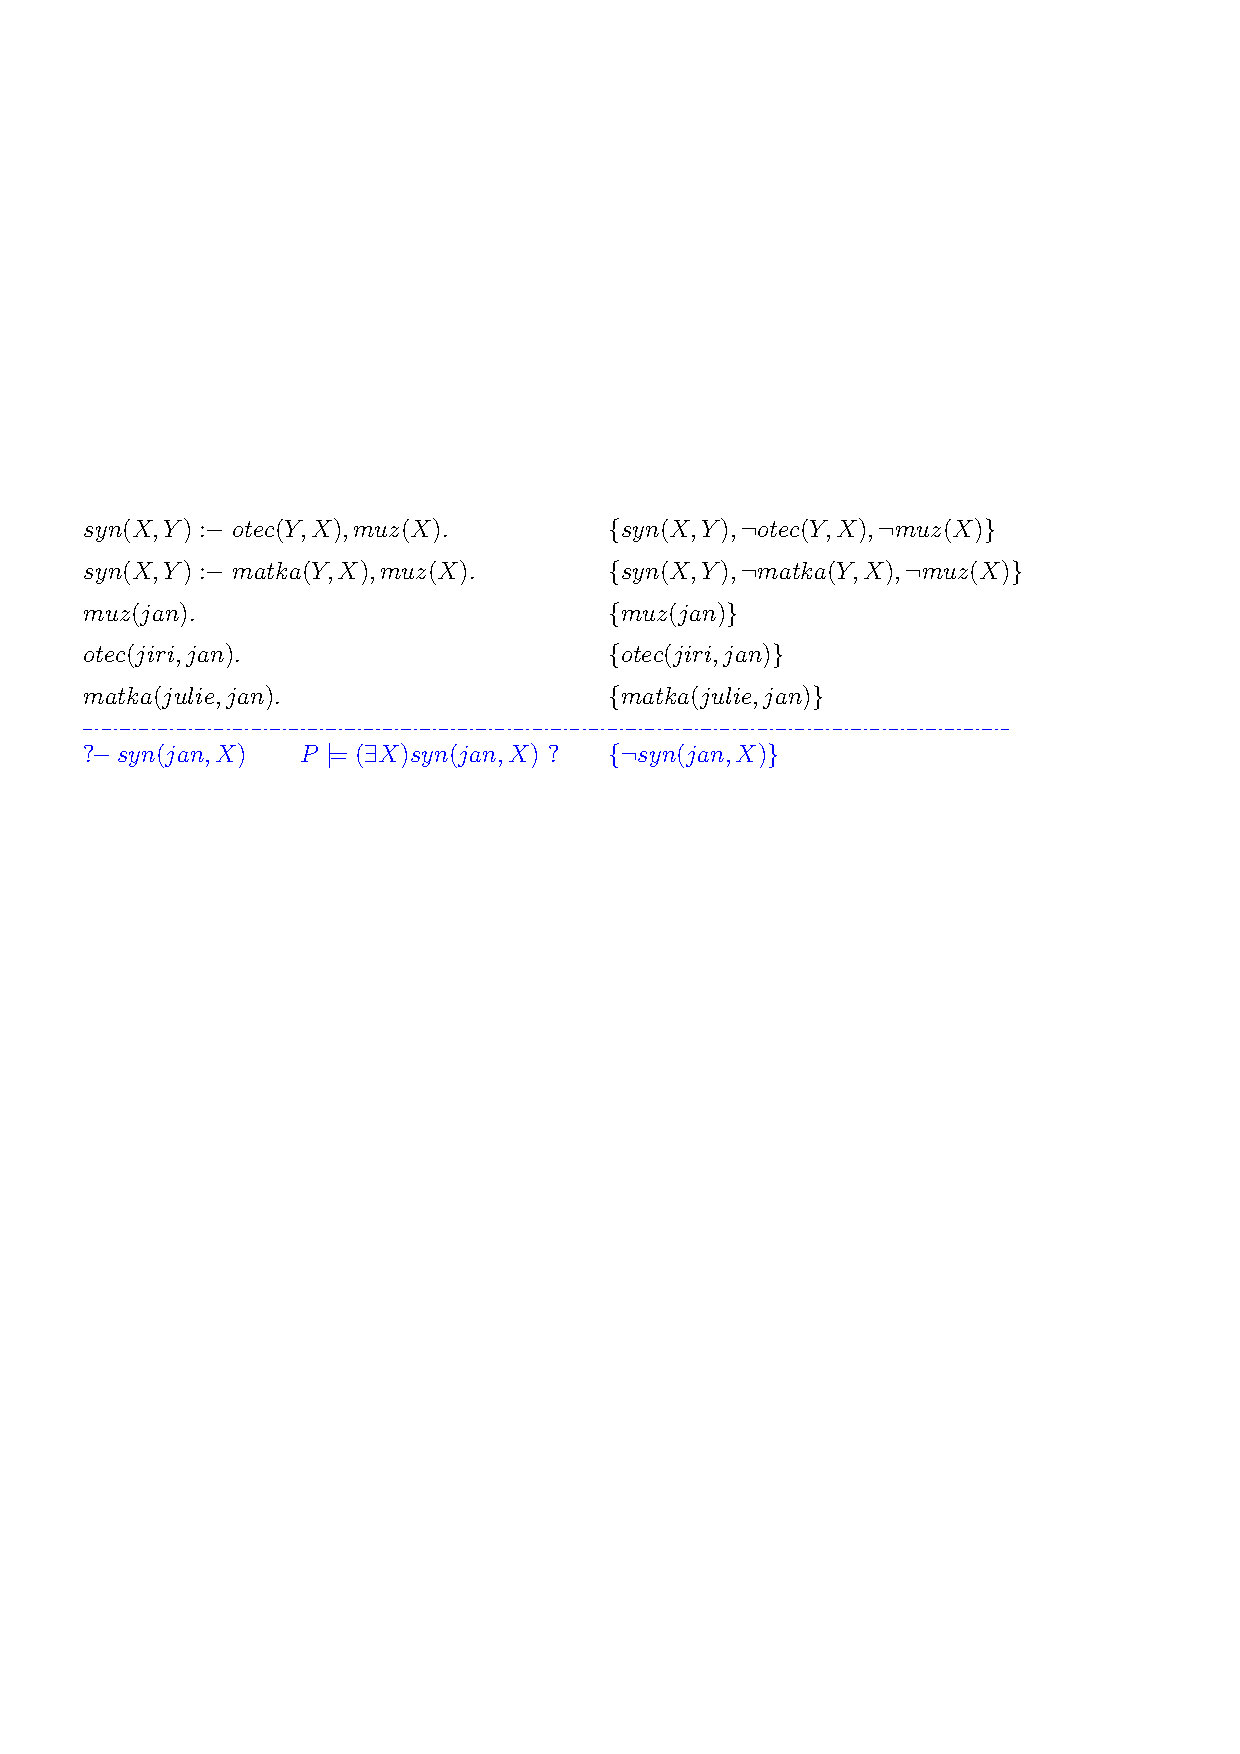
\includegraphics[scale=0.7]{files/rezolucePLprogram}}
    \bigskip
    
    {\it Zajímá nás, zda daný \myblue{existenční dotaz} vyplývá z daného programu.}%, navíc to chceme doložit \myblue{výstupní substitucí}.
    \medskip
    
    {\bf \myblue{Důsledek}}\ \ {\it Pro program $P$ a cíl $G=\{\neg A_1, \dots, \neg A_n\}$ v proměnných $X_1,\dots,X_m$
    
    \vspace{-0mm}
    \begin{enumerate}
    \item[$(1)$] $P \models (\exists X_1)\dots(\exists X_m)(A_1\mand \dots \mand A_n)$, právě když
    \smallskip
    
    \item[$(2)$] $\square$ lze odvodit LI-rezolucí z $P\cup\{G\}$ začínající (variantou) cíle $G$.
    \end{enumerate}}
    
    
    %%%%%%%%%%%%%%%%%%%%%%%%%%%%%%%%%%%%%%%%%%%%%%%%%%%%%%5
    
    \subsubsection*{LI-rezoluce nad programem}
    {\it Je-li odpověď na dotaz kladná, chceme navíc znát výstupní substituci.}
    \medskip
    
    \mdef{Výstupní substituce} $\sigma$ LI-rezoluce $\square$ z $P\cup\{G\}$ začínající $G=\{\neg A_1,\dots,\neg A_n\}$
    \smallskip
    
    je složení \myblue{mgu} v jednotlivých krocích (jen na proměnné v $G$). Platí,
    \vspace{-2mm}
    \mygreen{$$P \models (A_1 \mand \dots \mand A_n)\sigma.$$}
    
    \vspace{-2mm}
    
    \centerline{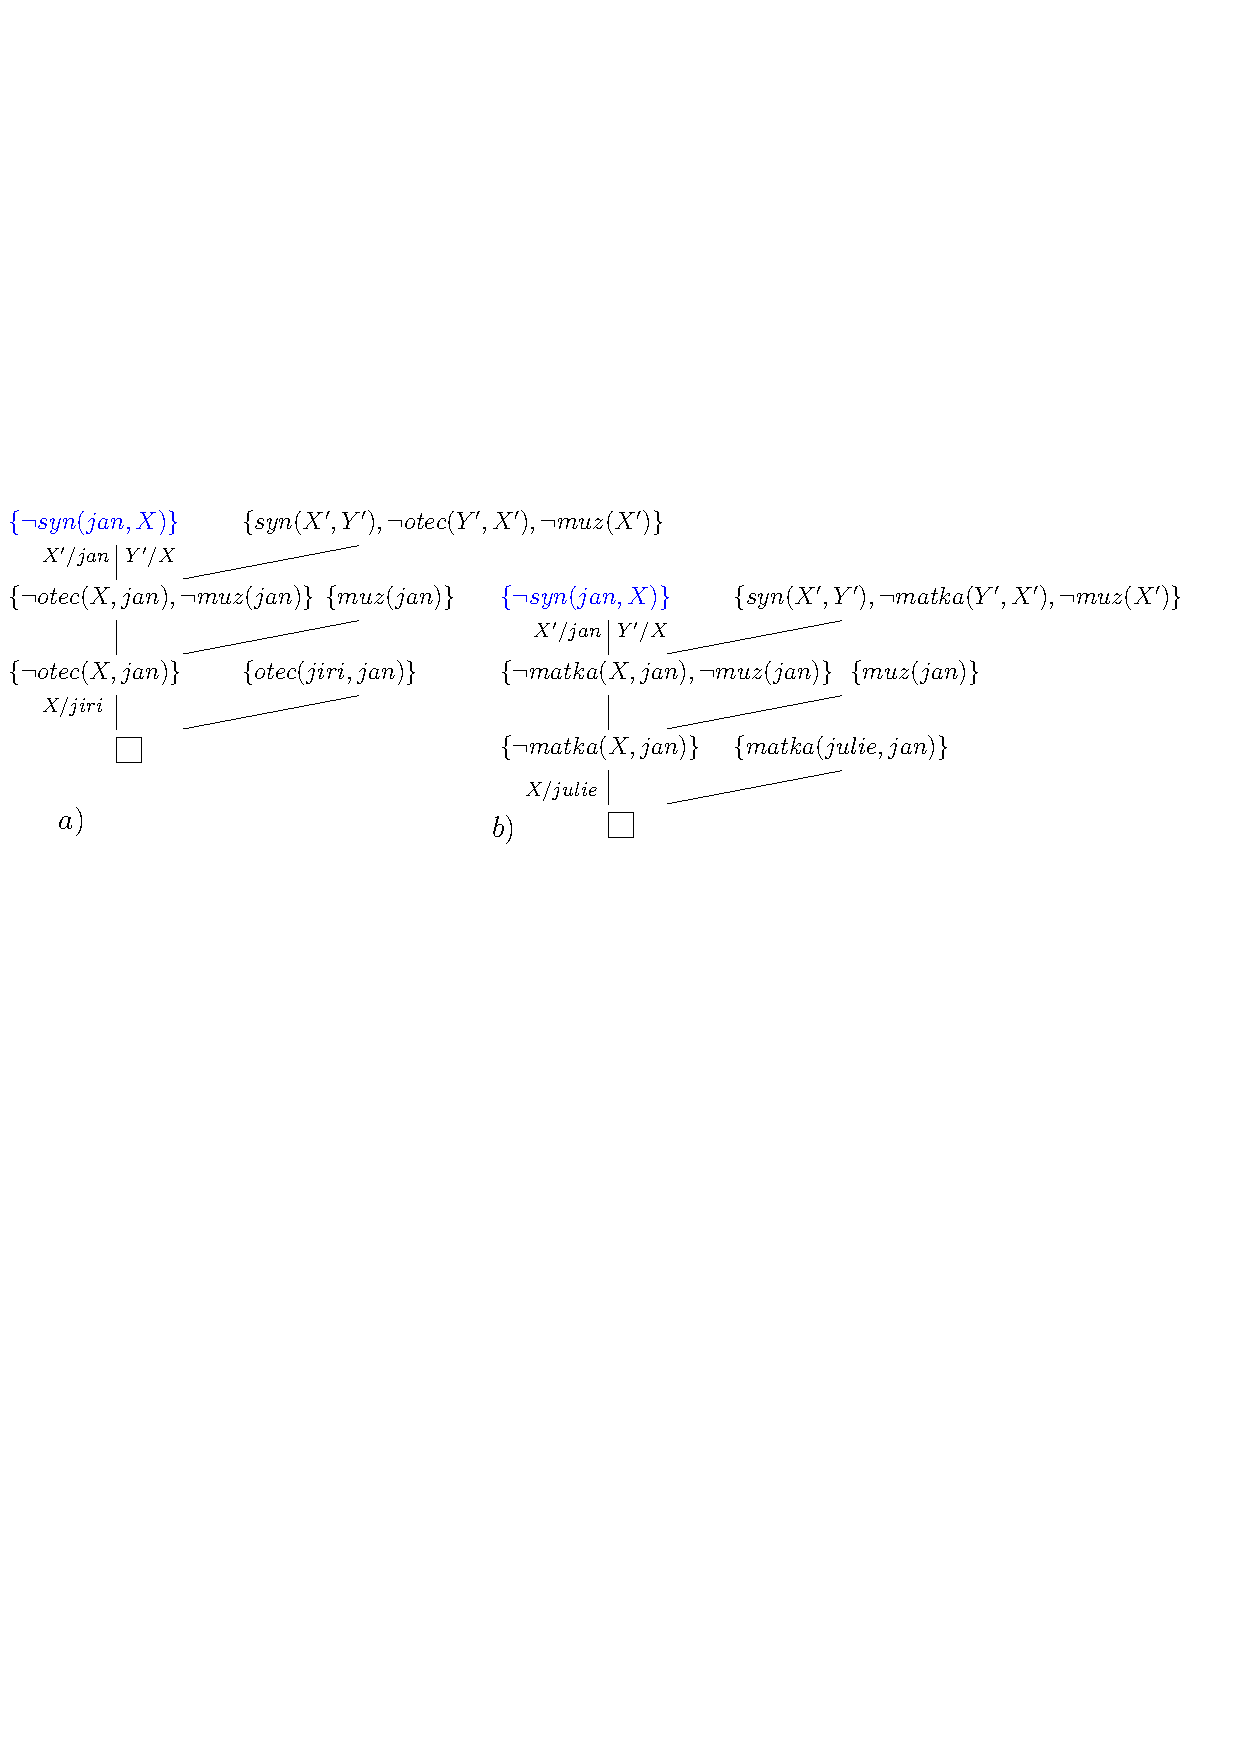
\includegraphics[scale=0.63]{files/rezolucePLprogramLI}}
    \bigskip
    
    Výstupní substituce $a)$ $X=jiri$,\ \ $b)$ $X=julie$.
    
    
% :from slides



